\documentclass[10pt,UTF8]{ctexart}


\usepackage[margin=2cm,a4paper]{geometry}
%\usepackage[left=0.75in,top=0.6in,right=0.75in,bottom=1.0in,a4paper]{geometry}

\setmainfont{Caladea}
%% 也可以選用其它字庫:
% \setCJKmainfont[%
%   ItalicFont=AR PL KaitiM GB,
%   BoldFont=Noto Sans CJK SC,
% ]{Noto Serif CJK SC}
% setCJKsansfont{Noto Sans CJK SC}
% \renewcommand{\kaishu}{\CJKfontspec{AR PL KaitiM GB}}

% 繁體中文
\setCJKmainfont[Path=fonts/ ]{NotoSansTC-Medium.otf}

\usepackage{minted}
\usepackage[breaklinks]{hyperref}

% Picture
% 導言區的此三行無變化
\usepackage{graphicx}
\usepackage{float} 
\usepackage{subfigure}
% 以下是新增的自定義格式更改
\usepackage[]{caption2} %新增調用的宏包
\renewcommand{\figurename}{Fig.} %重定義編號前綴詞
\renewcommand{\captionlabeldelim}{.~} %重定義分隔符
 %\roman 是羅馬數字編號,\alph是默認的字母編號,\arabic是阿拉伯數字編號,可按需替換下一行的相應位置
\renewcommand{\thesubfigure}{(\roman{subfigure})}%此外,還可設置圖編號顯示格式,加括號或者不加括號
\makeatletter \renewcommand{\@thesubfigure}{\thesubfigure \space}%子圖編號與名稱的間隔設置
\renewcommand{\p@subfigure}{} \makeatother

% Math
\usepackage {mathtools}
\usepackage{amssymb}

% Code
\usepackage{listings}
\usepackage{xcolor}
\lstset{
    % backgroundcolor=\color{red!50!green!50!blue!50},
    % 程式碼塊背景色為淺灰色
    rulesepcolor= \color{gray}, % 程式碼塊邊框顏色
    breaklines=true,  % 程式碼過長則換行
    numbers=left, % 行號在左側顯示
    numberstyle= \small,% 行號字型
    % eywordstyle= \color{red,% 關鍵字顏色
    commentstyle=\color{gray}, % 註釋顏色
    frame=shadowbox % 用方框框住程式碼塊
    }

\usepackage{hyperref}

\title{算法分析和複雜性理論}
\author{干皓丞,2101212850, 信息工程學院}

\begin{document}
\maketitle


\section{作業目標與章節摘要}

1. LeetCode 692. Top K Frequent Words 前K個高頻單詞

2. LeetCode 787. Cheapest Flights Within K Stops, K 站中轉內最便宜的航班

3. LeetCode 934. Shortest Bridge 最短的橋


\section{作業內容概述}

作業可以從 GitHub 下的 kancheng/kan-cs-report-in-2022 專案找到,作業程式碼與文件目錄為 kan-cs-report-in-2022/AATCC/lab-report/。實際執行的環境與實驗設備為 Google 的 Colab 、MacBook Pro (Retina, 15-inch, Mid 2014) 、 Acer Aspire R7 與 HP Victus (Nvidia GeForce RTX 3060)。

本作業 GitHub 專案為 kancheng/kan-cs-report-in-2022 下的 AATCC` 的目錄。程式碼可以從 code 目錄下可以找到 *.pynb,內容包含上次課堂練習、LeetCode 範例思路整理與作業。

https://github.com/kancheng/kan-cs-report-in-2022/tree/main/AATCC

\begin{figure}[H]
\centering 

\includegraphics[width=0.30\textwidth]{aatccqr.png} 
\caption{作業專案位置}
\label{Test}
\end{figure}


1. LeetCode : https://leetcode.com/

2. LeetCode CN : https://leetcode-cn.com/

3. OnlineGDB : https://www.onlinegdb.com/ 

LeetCode 的平台部分, CN 的平台有針對簡體中文使用者進行處理,包含中英文切換等功能。OnlineGDB 則可線上進行簡易的環境測試,其程式碼涵蓋 C, C++, C\#, Java, Python, JS, Rust, Go。

\newpage

\section{LeetCode 692. Top K Frequent Words 前K個高頻單詞}

\subsection{LeetCode 692. 題目}

Given an array of strings words and an integer k, return the k most frequent strings.

Return the answer sorted by the frequency from highest to lowest. Sort the words with the same frequency by their lexicographical order.

給定一個單詞列表 words 和一個整數 k ,返回前 k 個出現次數最多的單詞。

返回的答案應該按單詞出現頻率由高到低排序。如果不同的單詞有相同出現頻率, 按字典順序 排序。

Example 1:

\begin{lstlisting}[language={python}]
Input: words = ["i","love","leetcode","i","love","coding"], k = 2
Output: ["i","love"]
Explanation: "i" and "love" are the two most frequent words.
Note that "i" comes before "love" due to a lower alphabetical order.
解析: "i" 和 "love" 為出現次數最多的兩個單詞,均為2次。注意,按字母順序 "i" 在 "love" 之前。
\end{lstlisting}


Example 2:

\begin{lstlisting}[language={python}]
Input: words = ["the","day","is","sunny","the","the","the","sunny","is","is"], k = 4
Output: ["the","is","sunny","day"]
Explanation: "the", "is", "sunny" and "day" are the four most frequent words, with the number of occurrence being 4, 3, 2 and 1 respectively.
解析: "the", "is", "sunny" 和 "day" 是出現次數最多的四個單詞,出現次數依次為 4, 3, 2 和 1 次。
\end{lstlisting}


Constraints:

1. 1 <= words.length <= 500

2. 1 <= words[i] <= 10

3. words[i] consists of lowercase English letters.

4. k is in the range [1, The number of unique words[i]]

words[i] 由小寫英文字母組成。

k 的取值範圍是 [1, 不同 words[i] 的數量]

Follow-up: Could you solve it in O(n log(k)) time and O(n) extra space?

進階:嘗試以 O(n log k) 時間複雜度和 O(n) 空間複雜度解決。


\subsection{LeetCode 692. 思路總結}

維護一個長度為 k 的最大堆,先按照頻率排,如果頻率相同再按照字母順序排。最後輸出依次將優先隊列裡面的元素 pop 出來即可。

\subsection{LeetCode 692. Code 範例}

\begin{lstlisting}[language={python}]
from typing import List
class Solution:
    def topKFrequent(self, words: List[str], k: int) -> List[str]:
        q = []
        dic = collections.defaultdict(int)
        for word in words:
            dic[word] += 1
        
        for key, val in dic.items():
            heapq.heappush(q, (-val, key))
        
        return [heapq.heappop(q)[1] for i in range(k)]
\end{lstlisting}

\subsection{LeetCode 692. 結果}

\begin{figure}[H]
\centering 
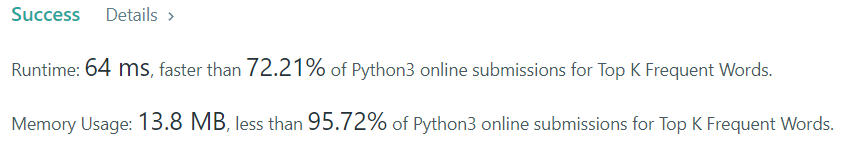
\includegraphics[width=0.80\textwidth]{lc-692-o.png} 
\caption{LeetCode 692 結果}
\label{Test}
\end{figure}


\newpage

\section{LeetCode 787. Cheapest Flights Within K Stops, K 站中轉內最便宜的航班}

\subsection{LeetCode 787. 題目}

There are n cities connected by some number of flights. You are given an array flights where flights[i] = [fromi, toi, pricei] indicates that there is a flight from city fromi to city toi with cost pricei.

You are also given three integers src, dst, and k, return the cheapest price from src to dst with at most k stops. If there is no such route, return -1.

有 n 個城市通過一些航班連接。給你一個數組 flights ,其中 flights[i] = [fromi, toi, pricei] ,表示該航班都從城市 fromi 開始,以價格 pricei 抵達 toi。

現在給定所有的城市和航班,以及出發城市 src 和目的地 dst,你的任務是找到出一條最多經過 k 站中轉的路線,使得從 src 到 dst 的 價格最便宜 ,並返回該價格。如果不存在這樣的路線,則輸出 -1。

\begin{figure}[H]
\centering 
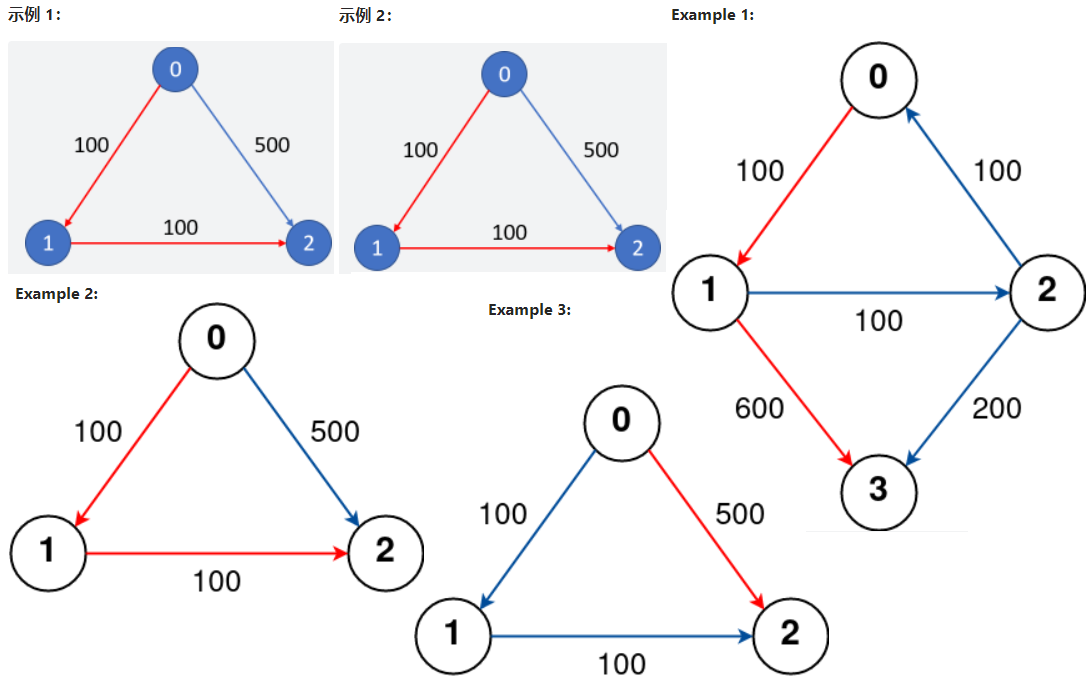
\includegraphics[width=0.80\textwidth]{lc-787-p-example.png} 
\caption{Example}
\label{Test}
\end{figure}

Example 1:

\begin{lstlisting}[language={python}]
Input: n = 4, flights = [[0,1,100],[1,2,100],[2,0,100],[1,3,600],[2,3,200]], src = 0, dst = 3, k = 1
Output: 700
Explanation:
The graph is shown above.
The optimal path with at most 1 stop from city 0 to 3 is marked in red and has cost 100 + 600 = 700.
Note that the path through cities [0,1,2,3] is cheaper but is invalid because it uses 2 stops.
\end{lstlisting}

Example 2:

\begin{lstlisting}[language={python}]
Input: n = 3, flights = [[0,1,100],[1,2,100],[0,2,500]], src = 0, dst = 2, k = 1
Output: 200
Explanation:
The graph is shown above.
The optimal path with at most 1 stop from city 0 to 2 is marked in red and has cost 100 + 100 = 200.
\end{lstlisting}

Example 3:

\begin{lstlisting}[language={python}]
Input: n = 3, flights = [[0,1,100],[1,2,100],[0,2,500]], src = 0, dst = 2, k = 0
Output: 500
Explanation:
The graph is shown above.
The optimal path with no stops from city 0 to 2 is marked in red and has cost 500.
\end{lstlisting}

示例 1:

\begin{lstlisting}[language={python}]
輸入: 
n = 3, edges = [[0,1,100],[1,2,100],[0,2,500]]
src = 0, dst = 2, k = 1
輸出: 200
解釋: 
城市航班圖如下
從城市 0 到城市 2 在 1 站中轉以內的最便宜價格是 200,如圖中紅色所示。
\end{lstlisting}

示例 2:

\begin{lstlisting}[language={python}]
輸入: 
n = 3, edges = [[0,1,100],[1,2,100],[0,2,500]]
src = 0, dst = 2, k = 0
輸出: 500
解釋: 
城市航班圖如下
從城市 0 到城市 2 在 0 站中轉以內的最便宜價格是 500,如圖中藍色所示。
\end{lstlisting}


Constraints:

1. 1 <= n <= 100

2. 0 <= flights.length <= (n * (n - 1) / 2)

3. flights[i].length == 3

4. 0 <= fromi, toi < n

5. $from_i$ != $to_i$

6. 1 <= pricei <= $10^4$

7. There will not be any multiple flights between two cities.(航班沒有重複,且不存在自環)

8. 0 <= src, dst, k < n
- src != dst



\subsection{LeetCode 787. 思路總結}

堆疊或者動態規劃

\subsection{LeetCode 787. Code 範例}

\begin{lstlisting}[language={python}]
class Solution:
    def findCheapestPrice(self, n: int, flights: List[List[int]], src: int, dst: int, K: int) -> int:
        dp = [float('inf') for _ in range(n)]
        dp[src] = 0
        for i in range(K+1):
            tmp = dp[:]
            for u, v, w in flights:
                dp[v] = min(dp[v],tmp[u]+w)
        return dp[dst] if dp[dst] != float('inf') else -1
\end{lstlisting}

\begin{lstlisting}[language={python}]
class Solution:
    def findCheapestPrice(self, n: int, flights: List[List[int]], src: int, dst: int, K: int) -> int:
        if src == dst: return 0
        graph = collections.defaultdict(dict)
        for start,end,cost in flights:
            graph[start][end] = cost

        queue = [(0,0,src)]
        while queue:
            cost, k, end = heapq.heappop(queue)
            if k > K+1 : continue
            if end == dst: return cost
            for key, val in graph[end].items():
                heapq.heappush(queue,(cost+val,k+1,key))
        return -1
\end{lstlisting}

\begin{lstlisting}[language={python}]
from collections import defaultdict
from queue import PriorityQueue
from typing import List, Dict

class Solution:
    def findCheapestPrice(self, n: int, flights: List[List[int]], src: int, dst: int, k: int) -> int:
        graph = self.build_graph(flights)

        prices = [float('inf')] * n
        stops = [float('inf')] * n

        prices[src] = 0
        stops[src] = 0

        queue = PriorityQueue()
        start_distance, start_stop = 0, 0
        queue.put(item=(start_distance, start_stop, src))
        while not queue.empty():
            node_price, node_stop, node_id = queue.get()
            if dst == node_id:
                return node_price
            if node_stop == k + 1:
                continue
            for neighbour, weight in graph[node_id].items():
                new_price = node_price + weight
                new_stop = node_stop + 1
                if new_price < prices[neighbour] or new_stop < stops[neighbour]:
                    queue.put(item=(new_price, new_stop, neighbour))
                    prices[neighbour] = new_price
                    stops[neighbour] = new_stop

        return -1 if prices[dst] == float("inf") else prices[dst]

    def build_graph(self, fs: List) -> Dict[int, Dict[int, int]]:
        graph = defaultdict(dict)
        for start, end, weight in fs:
            graph[start][end] = weight
        return graph
\end{lstlisting}



\subsection{LeetCode 787. 結果}

\begin{figure}[H]
\centering 
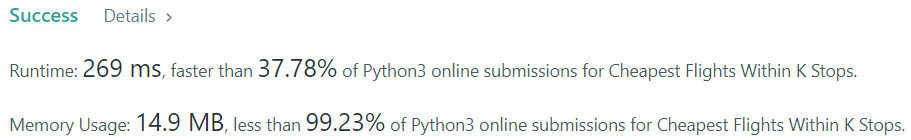
\includegraphics[width=0.80\textwidth]{lc-787-o.png} 
\caption{LeetCode 787 結果}
\label{Test}
\end{figure}


\newpage

\section{LeetCode 934. Shortest Bridge 最短的橋}

\subsection{LeetCode 934. 題目}

You are given an n x n binary matrix grid where 1 represents land and 0 represents water.

An island is a 4-directionally connected group of 1's not connected to any other 1's. There are exactly two islands in grid.

You may change 0's to 1's to connect the two islands to form one island.

Return the smallest number of 0's you must flip to connect the two islands.

在給定的二維二進制數組 A 中,存在兩座島。 (島是由四面相連的 1 形成的一個最大組。)

現在,我們可以將 0 變為 1,以使兩座島連接起來,變成一座島。

返回必須翻轉的 0 的最小數目。 (可以保證答案至少是 1 。)

Example 1:

\begin{lstlisting}[language={python}]
Input: grid = [[0,1],[1,0]]
Output: 1
\end{lstlisting}

Example 2:

\begin{lstlisting}[language={python}]
Input: grid = [[0,1,0],[0,0,0],[0,0,1]]
Output: 2
\end{lstlisting}

Example 3:

\begin{lstlisting}[language={python}]
Input: grid = [[1,1,1,1,1],[1,0,0,0,1],[1,0,1,0,1],[1,0,0,0,1],[1,1,1,1,1]]
Output: 1
\end{lstlisting}

Constraints:

1. n == grid.length == grid[i].length

2. 2 <= n <= 100

3. grid[i][j] is either 0 or 1.

4. There are exactly two islands in grid.

\begin{lstlisting}[language={python}]
/* 思路: DFS + BFS */
/* 先用深度優先搜索DFS, 找到第1個島嶼, 將島嶼元素置為2, 併入隊   */
/* 再用廣度優先搜索BFS, 從第1個島嶼元素開始向外尋找, 找到的0置為2 */
/* 當找到第一個1時, 就返回尋找的路徑step                       */

/* 隊列結構體定義 */
typedef struct {
    int x;
    int y;
    int step;
} Queue;

/* DFS 尋找第一個島嶼元素 */
void dfs(int **A, int ASize, int i, int j, Queue *Q, int *rear) {
    if (i < 0 || i >= ASize || j < 0 || j >= ASize || A[i][j] != 1) {
        return;
    }
    /* 元素置為2, 併入隊, step置為0 */
    A[i][j]           = 2;
    Q[(*rear)].x      = i;
    Q[(*rear)].y      = j;
    Q[(*rear)++].step = 0;

    /* 上下左右繼續尋找 */
    dfs(A, ASize, i - 1, j, Q, rear); 
    dfs(A, ASize, i + 1, j, Q, rear);
    dfs(A, ASize, i, j - 1, Q, rear);
    dfs(A, ASize, i, j + 1, Q, rear);
    return;
}

int shortestBridge(int** A, int ASize, int* AColSize){
    Queue *Q = (Queue*)malloc(sizeof(Queue) * ASize * ASize);
    int front = 0;
    int rear  = 0;
    int find  = 0;
    int i, j, x, y, xx, yy, step;
    int xShift[] = {-1, 1,  0, 0};
    int yShift[] = { 0, 0, -1, 1};

    /* DFS第一個島嶼 */
    for (i = 0; i < ASize; i++) {
        for (j = 0; j < ASize; j++) {
            if (A[i][j] == 1) {
                dfs(A, ASize, i, j, Q, &rear);
                find = 1;
                break;
            }
        }
        /* 只尋找第一個島嶼 */
        if (find == 1) {
            break;
        }
    }

    /* BFS 第一個島嶼向外擴散 */
    while (front != rear) {
        x    = Q[front].x;
        y    = Q[front].y;
        step = Q[front++].step;

        /* 上下左右擴散 */
        for (i = 0; i < 4; i++) {
            xx = x + xShift[i];
            yy = y + yShift[i];
            if (xx < 0 || xx >= ASize || yy < 0 || yy >= ASize || A[xx][yy] == 2) {
                continue;
            }
            if (A[xx][yy] == 1) { /* 找到另一島嶼時, 返回step */
                return step;
            }
            A[xx][yy]      = 2; /* 將擴散到的0置為2, 併入隊 */
            Q[rear].x      = xx;
            Q[rear].y      = yy;
            Q[rear++].step = step + 1;
        }
    }
    free(Q);
    return step;
}
\end{lstlisting}


\subsection{LeetCode 934. 思路總結}

DFS + BFS

\subsection{LeetCode 934. Code 範例}

\begin{lstlisting}[language={python}]
from collections import deque
from typing import List
class Solution:
    def shortestBridge(self, grid: List[List[int]]) -> int:
        def dfs(grid, x, y):
            grid[x][y] = 0
            seen.append([x, y])
            seen_set.add(f'{x}#{y}')
            axis = [[x - 1, y], [x + 1, y], [x, y -1], [x, y + 1]]
            for x, y in axis:
                if 0 <= x < m and 0 <= y < n and grid[x][y] == 1:
                    dfs(grid, x, y)
        def bfs(grid, seen):
            seen = deque(seen)
            seen_other_flag = False
            level = 0
            while seen:
                for _ in range(len(seen)):
                    x, y = seen.popleft()
                    axis = [[x - 1, y], [x + 1, y], [x, y -1], [x, y + 1]]
                    for x, y in axis:
                        index = f'{x}#{y}'
                        if 0 <= x < m and 0 <= y < n and index not in seen_set:
                            if grid[x][y] == 0:
                                seen.append([x, y])
                                seen_set.add(f'{x}#{y}')
                            else:
                                return level
                level += 1
            return level
        seen = []
        seen_set = set()
        m = len(grid)
        n = len(grid[0])
        search_flag = 0
        for i in range(m):
            for j in range(n):
                if grid[i][j] == 1 and not search_flag:
                    dfs(grid, i, j)
                    search_flag = 1
        level = bfs(grid, seen)
        return level
\end{lstlisting}

\subsection{LeetCode 934. 結果}

\begin{figure}[H]
\centering 
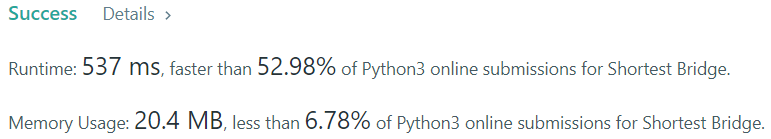
\includegraphics[width=0.80\textwidth]{lc-934-o.png} 
\caption{LeetCode 934 結果}
\label{Test}
\end{figure}



%\section{附錄}

% 數學意義說明

% $$\min \limits_{G}\max \limits_{D}{V_I(D,\ G)=V(D,G)-\lambda L_I(G,Q)}$$

%	\begin{lstlisting}[language={python}]

%	\end{lstlisting}

%\begin{enumerate}
%\item Y
%\item A
%\end{enumerate}

% \newpage

\clearpage

\end{document}